\documentclass[Arkitektur/System_main.tex]{subfiles}
\begin{document}
\subsubsection{RPiApp}
Dette er første udkast til applikationsmodellen for RPi - Vi arbejder stadig med at finde en løsning til at vise hvordan man skelner mellem user space og kernal space i applikationsmodellen. 
\\En anden ting er, at grænsefladerne og protokollerne er ikke helt opdateret og "slavecodes" er midlertidig navngivet. 
\\SlaveCode:
\\0xBD = BallDispenser
\\0XPS = Playerside (Ikke angivet en for hver playerside endnu) 
For andre kommandoer henvises til grænseflade afsnittet tabel \ref{tab:Protocol}

\begin{figure}[H]
    \centering
    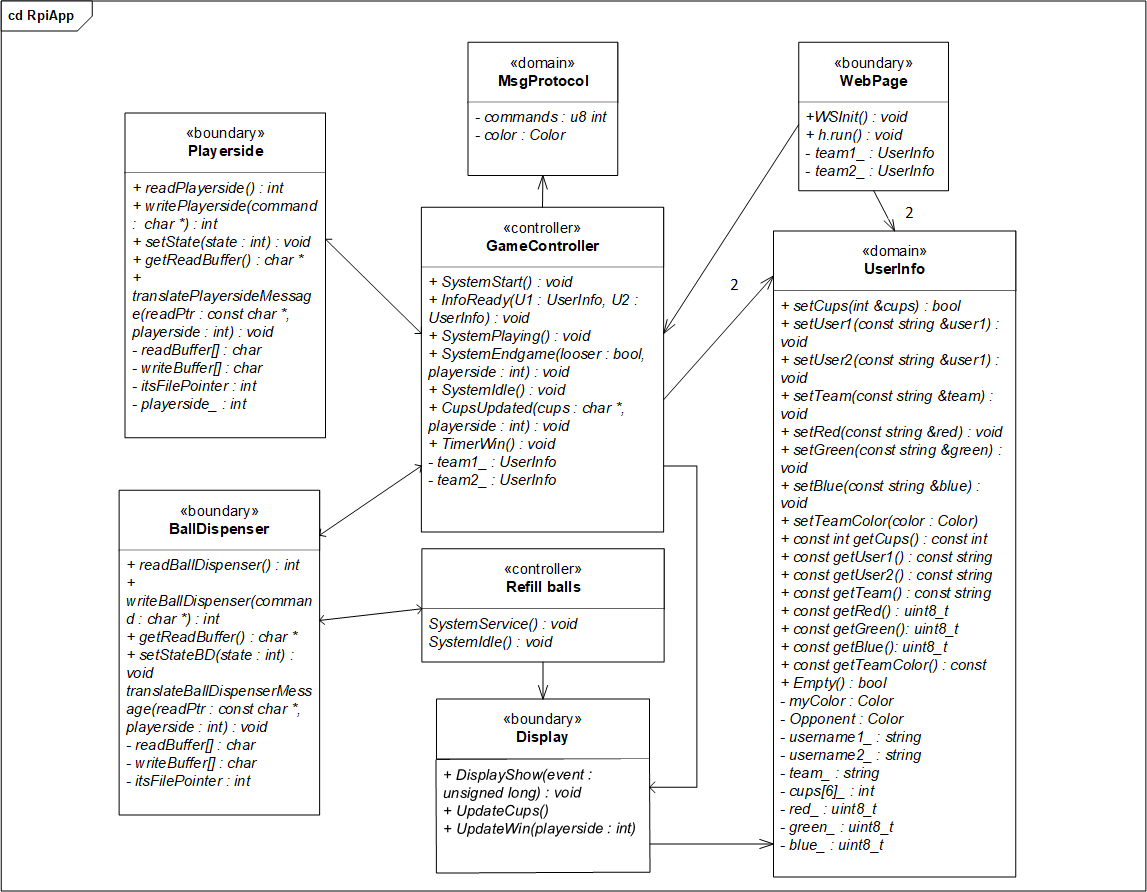
\includegraphics[width=\textwidth]{Arkitektur/Softwarearkitektur/Applikationsmodel/RPi/graphics_RPi/Class.png}
    \caption{Klassediagram for RPi}
    \label{fig:CD_RPI}
\end{figure}

\textbf{Controller:  GameController}\\
GameController er den centrale klasse for alle use cases. Den sørger for at sende og modtage data gennem klassen I2C. Alt modtaget data bliver evalueret i GameController og sendt videre i overensstemmelse med protokollen og use case flow. Klassen varetager alt logikken og de flest beslutninger i systemet. 

\textbf{Boundary:  Display}\\
Klasse til at opdatere det fysiske display tilknyttet systemet. 

\textbf{Boundary:  WebPage}\\
Grænsefladen til brugeren, en hjemmeside som modtager brugernes information og lagre dem i UserInfo. 

\textbf{Domain:  UserInfo}\\
Hukommelse om brugerne, hold og antal kopper tilbage. Denne domæne klasse findes ikke i domænemodellen, men er en sammensætning af domæneklasserne players, teams og scoreboard. Der er to af denne klasse, da hvert hold har informationer, og vurderingen om hvem har vundet tages ud fra dette. 

\textbf{Boundary:  I2C\_Protocol}\\
Information om slavernes adresse og kommandoernes betydning og funktion. 

\textbf{Boundary:  I2C}\\
Modtager og sender data mellem de forskellige enheder. Master er RPi og slaverne: Playerside(1-2) og Coin dispenser. For at den kan læse værdien sendt gennem I2C bruger GameController de to drivere "KernalPlayerSide" og "KernalDispenser". 

\textbf{Boundary:  InterruptServiceDriver}\\
InterruptServiceDriver er ikke en klasse, men derimod en driver implementeret i kernalspace. Dets ansvar er at "vække" \space GameController i tilfælde af interrupts fra en slave. 


\textbf{Boundary:  KernalPlayerSide}\\
Driver til at læse/skrive til Playerside via I2C protokollen. Enten sendes information fra userspace til kernalspace, som så sendes videre til Playerside - ellers læses data fra Playerside i kernalspace og sendes videre til userspace. 

\textbf{Boundary:  KernalDispenser}\\
Driver til at læse/skrive til BoldDispenser via I2C protokollen. Enten sendes information fra userspace til kernalspace, som så sendes videre til BallDispenser - ellers læses data fra BoldDispenser i kernalspace og sendes videre til userspace. 

\textbf{Sekvensdiagram for UC1: GameController}\\
GameControlleren er logikken i systemet og tager alle de store beslutninger. Dens hovedfunktioner er at modtage data fra de enkelte delsystemer, som boldDispenser og Playerside, og agerer i forhold til dette. Hvis et af disse delsystemer ønsker at kommunikere med GameControlleren (RPi) sendes der et ekstern interrupt. GameController poller derefter delsystemerne: den spørger hvem som har sendt interruptet. Når den har fundet ud af dette, så spørger den om den data den ønsker at sende, og opdaterer de andre systemer i forhold til den data. 
\\GameController sender også hvilken stadie Playerside og BoldDispenser skal være i, fx når spillet startes skal de være i stadiet "Starting". 

\begin{figure}[H]
    \centering
    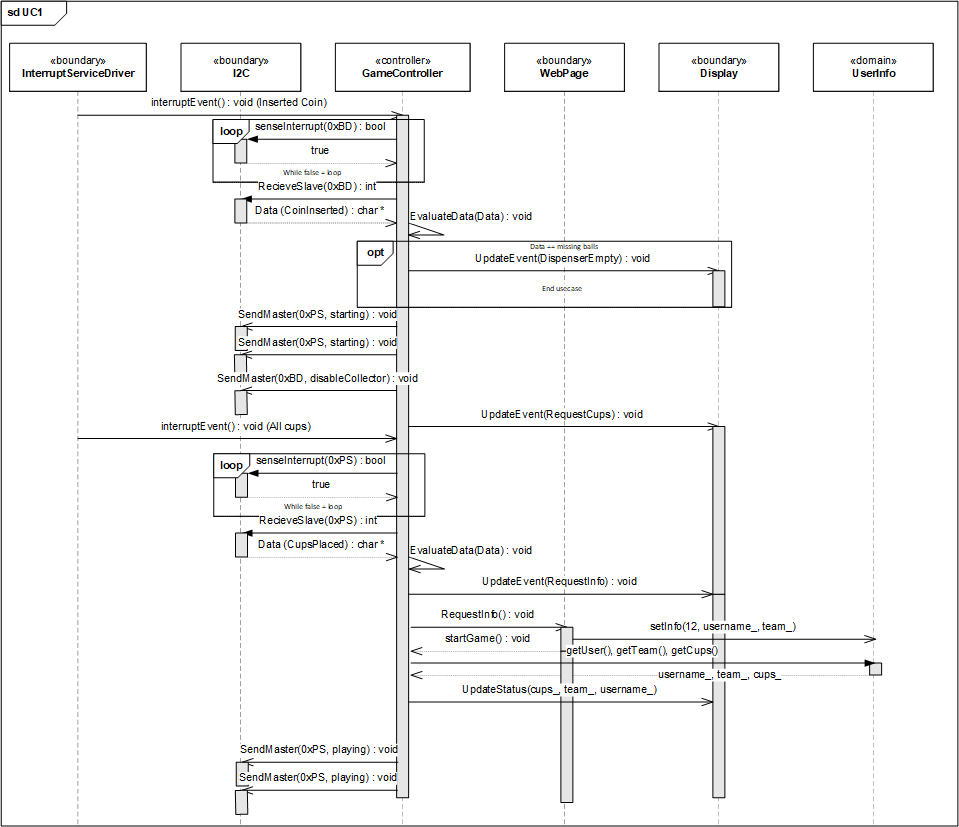
\includegraphics[width=\textwidth]{Arkitektur/Softwarearkitektur/Applikationsmodel/RPi/graphics_RPi/UC1_SD.png}
    \caption{Sekvensdiagram for UC1}
    \label{fig:UC1_SD_RPi}
\end{figure}

\textbf{Sekvensdiagram for UC2: GameController}\\
Spillet er startet og GameController har til opgave at hele tiden holde systemet opdateret i forhold til brugerens interaktioner. Hver gang brugeren fjerner en kop modtager RPi'en et interrupt (samme princip som i sekvensdigram for UC1). GameController opdaterer herefter displayet, således det som vises stemmer overens med det som sker på virkeligheden. 

\begin{figure}[H]
    \centering
    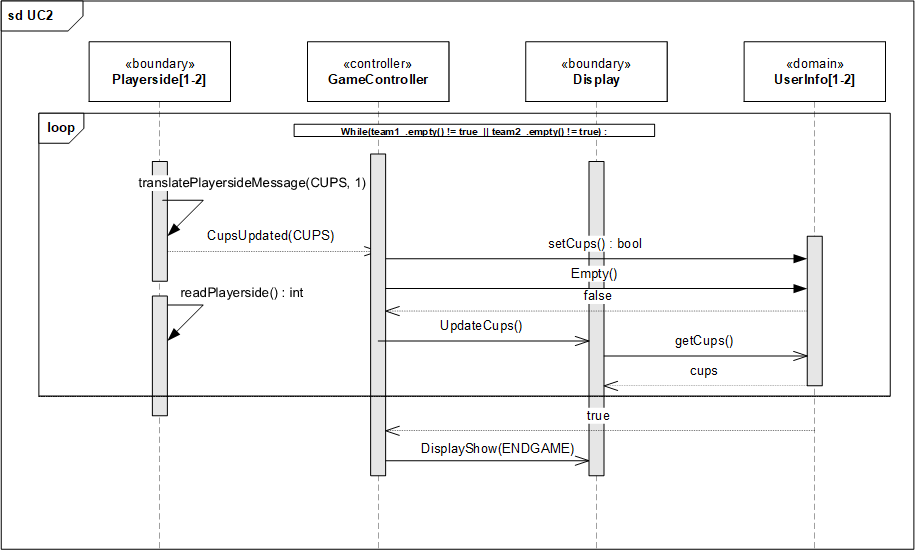
\includegraphics[width=\textwidth]{Arkitektur/Softwarearkitektur/Applikationsmodel/RPi/graphics_RPi/UC2_SD.png}
    \caption{Sekvensdiagram for UC2}
    \label{fig:UC2_SD_RPi}
\end{figure}

\newpage
\textbf{Sekvensdiagram for UC3: GameController}\\
GameControlleren har selv kontrolleret antallet af kopper tilbage på hvert side i forhold til det data, som har været sendt fra de to Playersides. Når den sidste kop er fjernet, sender den henholdsvis et signal til hver Playerside, hvem som har vundet og tabt. Dette vises på displayet i et specifikt tidsinterval, hvor derefter systemet vil gå i dvale og være klar til nye spillere. 

\begin{figure}[H]
    \centering
    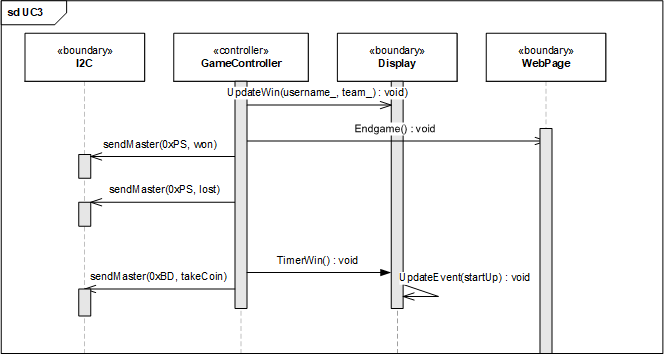
\includegraphics[width=\textwidth]{Arkitektur/Softwarearkitektur/Applikationsmodel/RPi/graphics_RPi/UC3_SD.png}
   \caption{Sekvensdiagram for UC3}
    \label{fig:UC3_SD_RPi}
\end{figure}

\newpage
\textbf{Sekvensdiagram for UC4: GameController}\\
I tilfælde af at boldDispenseren ikke har flere bolde, skal RPi'en udstede en besked til servicemedhjælperen og vente på at den er fyldt op (Eller har nok bolde til et spil).

\begin{figure}[H]
    \centering
    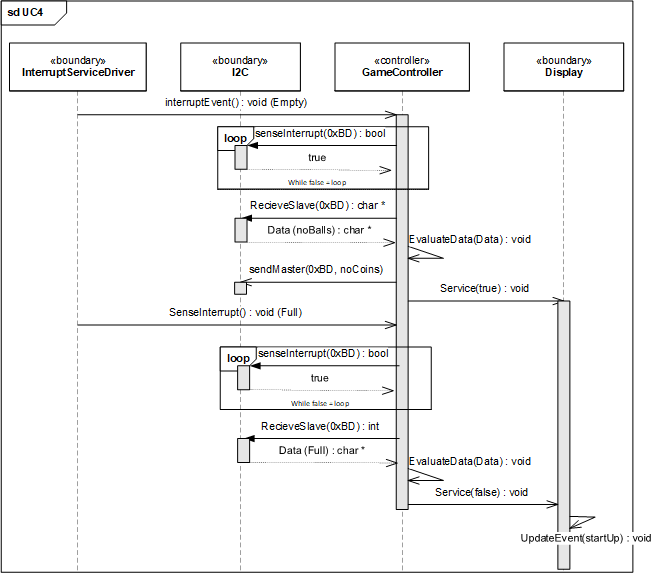
\includegraphics[width=\textwidth]{Arkitektur/Softwarearkitektur/Applikationsmodel/RPi/graphics_RPi/UC4_SD.png}
   \caption{Sekvensdiagram for UC4}
    \label{fig:UC4_SD_RPi}
\end{figure}

\textbf{Tilstandsmaskine: WebPage}\\
WebPage er brugerens mulighed for at gøre spillet personligt. Her indtastes holdnavne og brugernavne. WebPage er i en dvale tilstand indtil spillet starter. Her bliver brugeren spurgt om denne information gennem GUI'en og givet en IP-addresse via displayet. Når brugeren har trykket på "Start Game" udsteder den en konstant besked indtil spillet er slut. 

\begin{figure}[H]
    \centering
    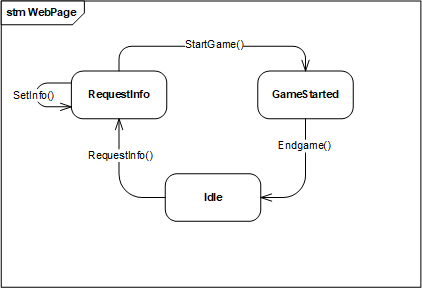
\includegraphics[width=\textwidth]{Arkitektur/Softwarearkitektur/Applikationsmodel/RPi/graphics_RPi/stm_web.png}
    \caption{Tilstandsmaskine for WebPage}
    \label{fig:stm_Web}
\end{figure}

\textbf{Tilstandsmaskine: Display}\\
Displayet viser konstant spillets status og fortæller brugerne hvad de skal gøre. Den skifter derved også tilstand i takt med spillets gang. 

\begin{figure}[H]
    \centering
    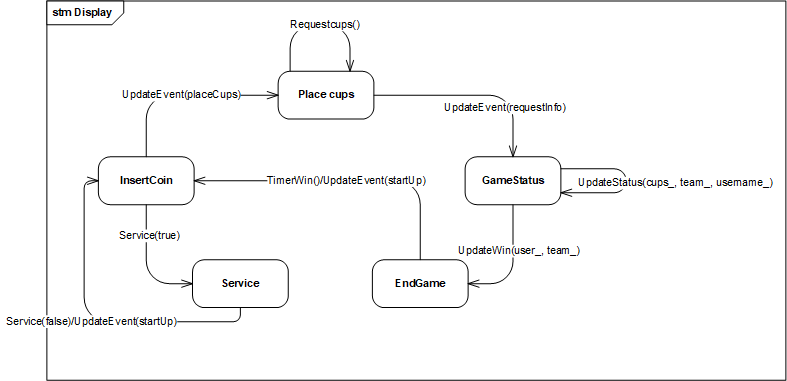
\includegraphics[width=\textwidth]{Arkitektur/Softwarearkitektur/Applikationsmodel/RPi/graphics_RPi/stm_disp.png}
    \caption{Tilstandsmaskine for Display}
    \label{fig:stm_disp}
\end{figure}

\textbf{Tilstandsmaskine: GameController}\\
Tilstandsmaskinen for GameController afspejler spillets gang. Den skifter konsekvent tilstand for hvert gang den får et interrupt og data fra de 3 delsystemer: Playerside(1 og 2) og BoldDispenser. 

\begin{figure}[H]
    \centering
    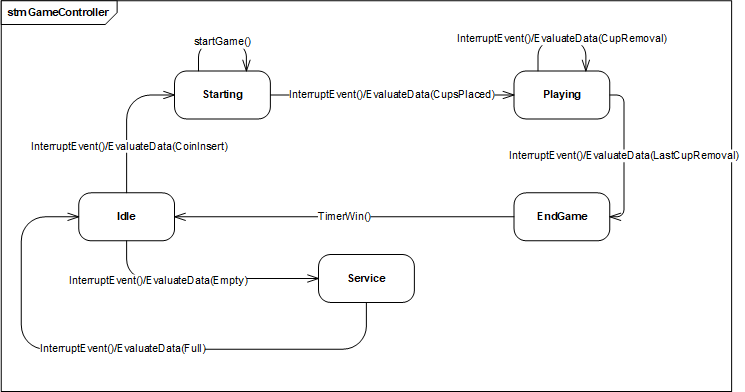
\includegraphics[width=\textwidth]{Arkitektur/Softwarearkitektur/Applikationsmodel/RPi/graphics_RPi/stm_Game.png}
    \caption{Tilstandsmaskine for GameController}
    \label{fig:stm_Game}
\end{figure}
\end{document}